%\iffalse %Beginn langer Kommentar
\chapter[Appendix]{Supplemental to Chapter 5\label{ch:app-pulsing}}

The following 4 Figures are from the supplemental material 
% of~\cname{Goering2022} which can be found here~\cite{Goering2022-supplemental}. 
The figures are recreated with permission from PRE.
% \section{Supplemental to Chapter 5}

\begin{figure*}[tbp]
  \centering
  % \tikzsetnextfilename{duty-m04}
{
  \small
%%%%%%%
% READ TABLE
%%%%%%%
\pgfplotstableread{SECTION/15_Figures/duty_fp_1000.dat}{\dataOne}
\pgfplotstableread{SECTION/15_Figures/duty_fp_5000.dat}{\dataTwo}
\pgfplotstableread{SECTION/15_Figures/duty_fp_10000.dat}{\dataThree}
%%%%%%%
% LINES FOR ALL GROUPPLOTS
%%%%%%%
\renewcommand{\tikzHelper}{
  \fill[fill=black!10!white] (axis cs:-80,0) rectangle (axis cs:0,1);

  \draw[dotted] (axis cs:0,0) -- (axis cs:0,1);
  \draw[dotted] (axis cs:50,0) -- (axis cs:50,1);
  \draw[dotted] (axis cs:100,0) -- (axis cs:100,1);
  \draw[dotted] (axis cs:-80,0.5) -- (axis cs:120,0.5);
  \draw[dotted] (axis cs:-80,0.5) -- (axis cs:120,0.5);
}

\renewcommand{\tmp}{04}

\begin{tikzpicture}
   \begin{groupplot}[%
       scale only axis,
       group style={
         group size= 2 by 3,
         group name=plots,
         vertical sep=4pt,%
         horizontal sep=8pt},%
       height=25mm,%
       width=64mm,%
        xticklabel style={
          /pgf/number format/fixed,
          /pgf/number format/precision=2
        }]

%%%%%%
%%% PLOT (1,1)
%%%%%%

   \nextgroupplot[%
     legend cell align={left},
     legend style={
        fill=black!10!white,
        font=\tiny,
        at={(0.02,0.95)},
        anchor=north west,
        /tikz/column 2/.style={column sep=1pt,},
        legend columns=2,
      },
     xticklabels={,,},
     % title={$\DV_{y}\,|\,\Dy = \SI{-0.06}{\milli\meter}$},%
     % title={Data for $y$-component},%
     title={ARF},%
     ylabel={$\sfrac{\DV_{j}}{\DV_{100,\text{max}}}$ },
 ]

      \tikzHelper

      \addlegendimage{empty legend}
      \addlegendimage{empty legend}

      \addplot[style100] table[x=dt, y=DV_y_m\tmp_100_m00] {\dataOne};
      \addplot[style90] table[x=dt, y=DV_y_m\tmp_090_m00] {\dataOne};
      \addplot[style80] table[x=dt, y=DV_y_m\tmp_080_m00] {\dataOne};
      \addplot[style70] table[x=dt, y=DV_y_m\tmp_070_m00] {\dataOne};
      \addplot[style60] table[x=dt, y=DV_y_m\tmp_060_m00] {\dataOne};
      \addplot[style50] table[x=dt, y=DV_y_m\tmp_050_m00] {\dataOne};


      \addlegendentry{\hspace{-6mm}\textbf{Duty \%}}
      \addlegendentry{\textbf{\phantom{a}}}
      \addlegendentry{100};
      \addlegendentry{90};
      \addlegendentry{80};
      \addlegendentry{70};
      \addlegendentry{60};
      \addlegendentry{50};


%%%%%%
%%% PLOT (1,2)
%%%%%%

   \nextgroupplot[%
     xticklabels={,,},
     yticklabels={,,},
     % title={Data for $z$-component}]%
     title={AS}]%

      \tikzHelper
      \draw[thick,|<->|] (axis cs:-80,0.25) -- (axis cs:0,0.25) node[midway, 
      above] {US off};

      \addplot[style100] table[x=dt, y=DV_z_m\tmp_100_m00] {\dataOne};
      \addplot[style90] table[x=dt, y=DV_z_m\tmp_090_m00] {\dataOne};
      \addplot[style80] table[x=dt, y=DV_z_m\tmp_080_m00] {\dataOne};
      \addplot[style70] table[x=dt, y=DV_z_m\tmp_070_m00] {\dataOne};
      \addplot[style60] table[x=dt, y=DV_z_m\tmp_060_m00] {\dataOne};
      \addplot[style50] table[x=dt, y=DV_z_m\tmp_050_m00] {\dataOne};

%%%%%%
%%% PLOT (2,1)
%%%%%%

   \nextgroupplot[%
     xticklabels={,,},
     ylabel={$\sfrac{\DV_{j}}{\DV_{100,\text{max}}}$ },
   ]

      \tikzHelper

      \addplot[style100] table[x=dt, y=DV_y_m\tmp_100_m00] {\dataTwo};
      \addplot[style90] table[x=dt, y=DV_y_m\tmp_090_m00] {\dataTwo};
      \addplot[style80] table[x=dt, y=DV_y_m\tmp_080_m00] {\dataTwo};

%%%%%%
%%% PLOT (2,2)
%%%%%%

   \nextgroupplot[%
     xticklabels={,,},
     yticklabels={,,},
   ]

      \tikzHelper

      \addplot[style100] table[x=dt, y=DV_z_m\tmp_100_m00] {\dataTwo};
      \addplot[style90] table[x=dt, y=DV_z_m\tmp_090_m00] {\dataTwo};
      \addplot[style80] table[x=dt, y=DV_z_m\tmp_080_m00] {\dataTwo};

%%%%%%
%%% PLOT (3,1)
%%%%%%

   \nextgroupplot[%
     ylabel={$\sfrac{\DV_{j}}{\DV_{100,\text{max}}}$ },
     xlabel={$10^{3}\,\sfrac{t}{t_{0}}$ },
   ]

      \tikzHelper

      \addplot[style100] table[x=dt, y=DV_y_m\tmp_100_m00] {\dataThree};
      \addplot[style90] table[x=dt, y=DV_y_m\tmp_090_m00] {\dataThree};
      \addplot[style80] table[x=dt, y=DV_y_m\tmp_080_m00] {\dataThree};
      \addplot[style70] table[x=dt, y=DV_y_m\tmp_070_m00] {\dataThree};
      \addplot[style60] table[x=dt, y=DV_y_m\tmp_060_m00] {\dataThree};
      \addplot[style50] table[x=dt, y=DV_y_m\tmp_050_m00] {\dataThree};

      \foreach \val/\index in
      {50/0.120,60/0.143,70/0.178,80/0.232,90/0.281,100/0.312,110/0.367,120/0.44} {
        \edef\temp{\noexpand
        \draw[] (axis cs:\val, 0) -- (axis cs:\val,\index);
        }
        \temp}


%%%%%%
%%% PLOT (3,2)
%%%%%%

   \nextgroupplot[%
     yticklabels={,,},
     xlabel={$10^{3}\,\sfrac{t}{t_{0}}$ },
     % title={$\Dy = \SI{-0.04}{\milli\meter}$}
   ]

      \tikzHelper

      \addplot[style100] table[x=dt, y=DV_z_m\tmp_100_m00] {\dataThree};
      \addplot[style90] table[x=dt, y=DV_z_m\tmp_090_m00] {\dataThree};
      \addplot[style80] table[x=dt, y=DV_z_m\tmp_080_m00] {\dataThree};
      \addplot[style70] table[x=dt, y=DV_z_m\tmp_070_m00] {\dataThree};
      \addplot[style60] table[x=dt, y=DV_z_m\tmp_060_m00] {\dataThree};
      \addplot[style50] table[x=dt, y=DV_z_m\tmp_050_m00] {\dataThree};


  \end{groupplot}

%%%%%%
%%% TEXT NEXT TO PLOTS
%%%%%%
  \node[above] at ($(plots c1r1.north west)!0.5!(plots c2r1.north east)$) 
  [yshift=10mm] {$\Dy = \SI{-0.\tmp}{\mm}$};


  \node[rotate=90] at (plots c2r2.east) [yshift=-5mm] 
  {$\fp=\sfrac{\fex}{\bullet}$};
  \node[rotate=90] at (plots c2r1.east) [yshift=-10mm] {1000};
  \node[rotate=90] at (plots c2r2.east) [yshift=-10mm] {5000};
  \node[rotate=90] at (plots c2r3.east) [yshift=-10mm] {10000};

\end{tikzpicture}
}

  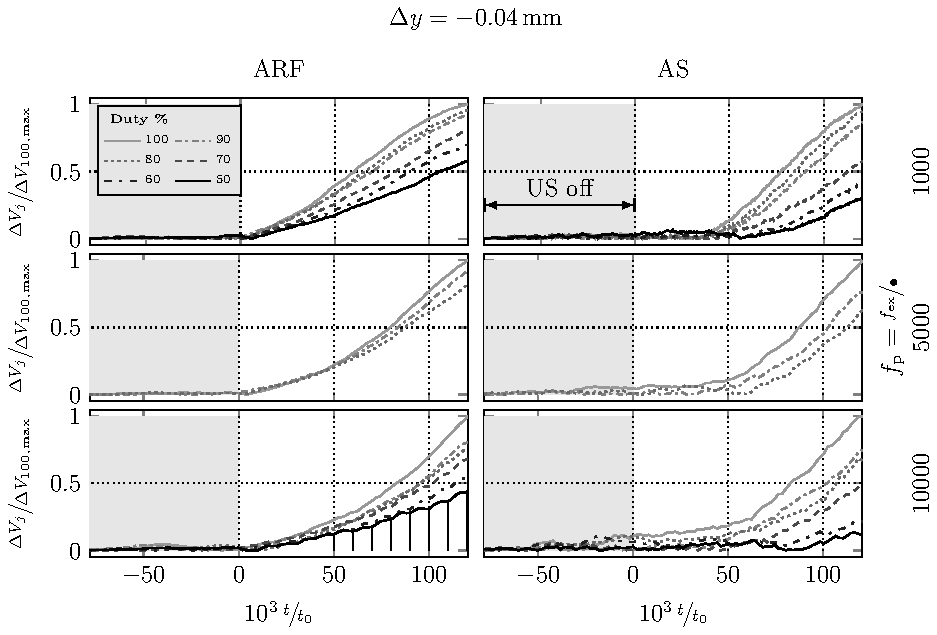
\includegraphics[]{External/duty-m04.pdf}
  \caption{Evolution of averaged voltage differences $\DV_{y}$ (left column; 
      ARF associated) and $\DV_{z}$ (right column; AS associated) for three 
      different pulsing frequencies $\fp$ and different duty percentages at 
      $\Dy=\SI{-0.04}{\mm}$. For the first row $\fp=\sfrac{\fex}{1'000}$, for 
      the second $\fp=\sfrac{\fex}{5'000}$, and for the last row 
      $\fp=\sfrac{\fex}{10'000}$. The data per plot is normalized to the 
      maximal amplitude of the data series with a duty percentage of 100\%. The 
      vertical solid lines in the bottom left plot mark the beginning of a new 
      pulsing cycle.
}
\end{figure*}
\newpage

\begin{figure*}[tbp]
  \centering
  % \tikzsetnextfilename{duty-m06}
{
  \small
%%%%%%%
% READ TABLE
%%%%%%%
\pgfplotstableread{SECTION/15_Figures/duty_fp_1000.dat}{\dataOne}
\pgfplotstableread{SECTION/15_Figures/duty_fp_5000.dat}{\dataTwo}
\pgfplotstableread{SECTION/15_Figures/duty_fp_10000.dat}{\dataThree}
%%%%%%%
% LINES FOR ALL GROUPPLOTS
%%%%%%%
\renewcommand{\tikzHelper}{
  \fill[fill=black!10!white] (axis cs:-80,0) rectangle (axis cs:0,1);

  \draw[dotted] (axis cs:0,0) -- (axis cs:0,1);
  \draw[dotted] (axis cs:50,0) -- (axis cs:50,1);
  \draw[dotted] (axis cs:100,0) -- (axis cs:100,1);
  \draw[dotted] (axis cs:-80,0.5) -- (axis cs:120,0.5);
  \draw[dotted] (axis cs:-80,0.5) -- (axis cs:120,0.5);
}

\renewcommand{\tmp}{06}

\begin{tikzpicture}
   \begin{groupplot}[%
       scale only axis,
       group style={
         group size= 2 by 3,
         group name=plots,
         vertical sep=4pt,%
         horizontal sep=8pt},%
       height=25mm,%
       width=64mm,%
        xticklabel style={
          /pgf/number format/fixed,
          /pgf/number format/precision=2
        }]

%%%%%%
%%% PLOT (1,1)
%%%%%%

   \nextgroupplot[%
     legend cell align={left},
     legend style={
        fill=black!10!white,
        font=\tiny,
        at={(0.02,0.95)},
        anchor=north west,
        /tikz/column 2/.style={column sep=1pt,},
        legend columns=2,
      },
     xticklabels={,,},
     % title={Data for $y$-component},%
     title={ARF},%
     ylabel={$\sfrac{\DV_{j}}{\DV_{100,\text{max}}}$ },
 ]

      \tikzHelper

      \addlegendimage{empty legend}
      \addlegendimage{empty legend}

      \addplot[style100] table[x=dt, y=DV_y_m\tmp_100_m00] {\dataOne};
      \addplot[style90] table[x=dt, y=DV_y_m\tmp_090_m00] {\dataOne};
      \addplot[style80] table[x=dt, y=DV_y_m\tmp_080_m00] {\dataOne};
      \addplot[style70] table[x=dt, y=DV_y_m\tmp_070_m00] {\dataOne};
      \addplot[style60] table[x=dt, y=DV_y_m\tmp_060_m00] {\dataOne};
      \addplot[style50] table[x=dt, y=DV_y_m\tmp_050_m00] {\dataOne};


      \addlegendentry{\hspace{-6mm}\textbf{Duty \% }}
      \addlegendentry{\textbf{\phantom{a}}}
      \addlegendentry{100};
      \addlegendentry{90};
      \addlegendentry{80};
      \addlegendentry{70};
      \addlegendentry{60};
      \addlegendentry{50};


%%%%%%
%%% PLOT (1,2)
%%%%%%

   \nextgroupplot[%
     xticklabels={,,},
     yticklabels={,,},
     % title={Data for $z$-component},
     title={AS},
   ]%

      \tikzHelper
      \draw[thick,|<->|] (axis cs:-80,0.25) -- (axis cs:0,0.25) node[midway, 
      above] {US off};

      \addplot[style100] table[x=dt, y=DV_z_m\tmp_100_m00] {\dataOne};
      \addplot[style90] table[x=dt, y=DV_z_m\tmp_090_m00] {\dataOne};
      \addplot[style80] table[x=dt, y=DV_z_m\tmp_080_m00] {\dataOne};
      \addplot[style70] table[x=dt, y=DV_z_m\tmp_070_m00] {\dataOne};
      \addplot[style60] table[x=dt, y=DV_z_m\tmp_060_m00] {\dataOne};
      \addplot[style50] table[x=dt, y=DV_z_m\tmp_050_m00] {\dataOne};

%%%%%%
%%% PLOT (2,1)
%%%%%%

   \nextgroupplot[%
     xticklabels={,,},
     ylabel={$\sfrac{\DV_{j}}{\DV_{100,\text{max}}}$ },
   ]

      \tikzHelper

      \addplot[style100] table[x=dt, y=DV_y_m\tmp_100_m00] {\dataTwo};
      \addplot[style90] table[x=dt, y=DV_y_m\tmp_090_m00] {\dataTwo};
      \addplot[style80] table[x=dt, y=DV_y_m\tmp_080_m00] {\dataTwo};

%%%%%%
%%% PLOT (2,2)
%%%%%%

   \nextgroupplot[%
     xticklabels={,,},
     yticklabels={,,},
   ]

      \tikzHelper

      \addplot[style100] table[x=dt, y=DV_z_m\tmp_100_m00] {\dataTwo};
      \addplot[style90] table[x=dt, y=DV_z_m\tmp_090_m00] {\dataTwo};
      \addplot[style80] table[x=dt, y=DV_z_m\tmp_080_m00] {\dataTwo};

%%%%%%
%%% PLOT (3,1)
%%%%%%

   \nextgroupplot[%
     ylabel={$\sfrac{\DV_{j}}{\DV_{100,\text{max}}}$ },
     xlabel={$10^{3}\,\sfrac{t}{t_{0}}$ },
   ]

      \tikzHelper

      \addplot[style100] table[x=dt, y=DV_y_m\tmp_100_m00] {\dataThree};
      \addplot[style90] table[x=dt, y=DV_y_m\tmp_090_m00] {\dataThree};
      \addplot[style80] table[x=dt, y=DV_y_m\tmp_080_m00] {\dataThree};
      \addplot[style70] table[x=dt, y=DV_y_m\tmp_070_m00] {\dataThree};
      \addplot[style60] table[x=dt, y=DV_y_m\tmp_060_m00] {\dataThree};
      \addplot[style50] table[x=dt, y=DV_y_m\tmp_050_m00] {\dataThree};


      \foreach \val/\index in 
      {50/0.108,60/0.132,70/0.158,80/0.188,90/0.221,100/0.252,110/0.301,120/0.35} {
        \edef\temp{\noexpand
        \draw[] (axis cs:\val, 0) -- (axis cs:\val,\index);
        }
        \temp}
%%%%%%
%%% PLOT (3,2)
%%%%%%

   \nextgroupplot[%
     yticklabels={,,},
     xlabel={$10^{3}\,\sfrac{t}{t_{0}}$ },
   ]

      \tikzHelper

      \addplot[style100] table[x=dt, y=DV_z_m\tmp_100_m00] {\dataThree};
      \addplot[style90] table[x=dt, y=DV_z_m\tmp_090_m00] {\dataThree};
      \addplot[style80] table[x=dt, y=DV_z_m\tmp_080_m00] {\dataThree};
      \addplot[style70] table[x=dt, y=DV_z_m\tmp_070_m00] {\dataThree};
      \addplot[style60] table[x=dt, y=DV_z_m\tmp_060_m00] {\dataThree};
      \addplot[style50] table[x=dt, y=DV_z_m\tmp_050_m00] {\dataThree};


  \end{groupplot}

%%%%%%
%%% TEXT NEXT TO PLOTS
%%%%%%
  \node[above] at ($(plots c1r1.north west)!0.5!(plots c2r1.north east)$) 
  [yshift=10mm] {$\Dy = \SI{-0.\tmp}{\mm}$};

  \node[rotate=90] at (plots c2r2.east) [yshift=-5mm] 
  {$\fp=\sfrac{\fex}{\bullet}$};
  \node[rotate=90] at (plots c2r1.east) [yshift=-10mm] {1000};
  \node[rotate=90] at (plots c2r2.east) [yshift=-10mm] {5000};
  \node[rotate=90] at (plots c2r3.east) [yshift=-10mm] {10000};

\end{tikzpicture}
}

  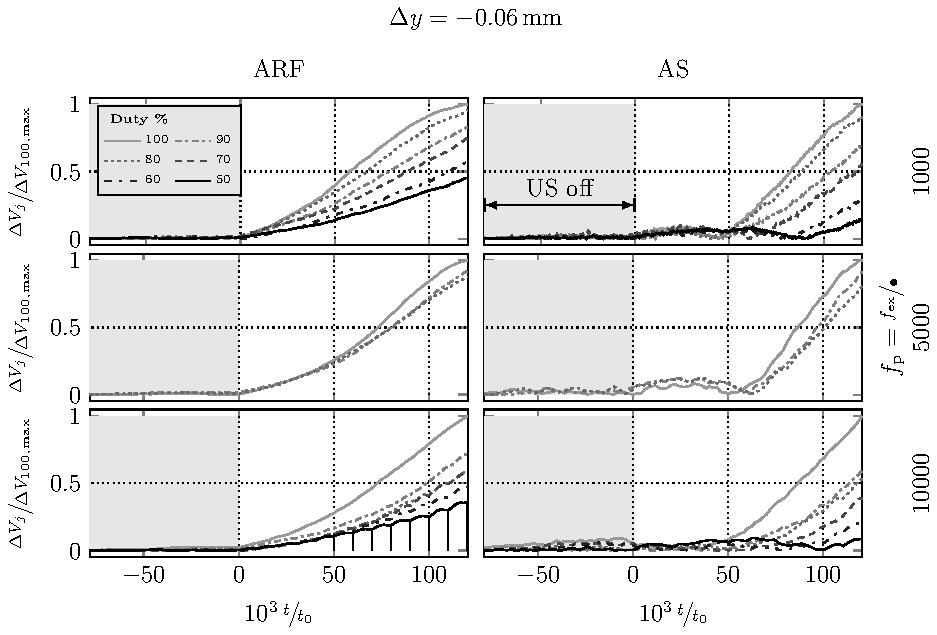
\includegraphics[]{External/duty-m06.pdf}
  \caption{Evolution of averaged voltage differences $\DV_{y}$ (left column; 
      ARF associated) and $\DV_{z}$ (right column; AS associated) for three 
      different pulsing frequencies $\fp$ and different duty percentages at 
      $\Dy=\SI{-0.06}{\mm}$. For the first row $\fp=\sfrac{\fex}{1'000}$, for 
      the second $\fp=\sfrac{\fex}{5'000}$, and for the last row 
      $\fp=\sfrac{\fex}{10'000}$. The data per plot is normalized to the 
      maximal amplitude of the data series with a duty percentage of 100\%. The 
      vertical solid lines in the bottom left plot mark the beginning of a new 
      pulsing cycle.
}
\end{figure*}

\newpage
\begin{figure*}[tbp]
  \centering
  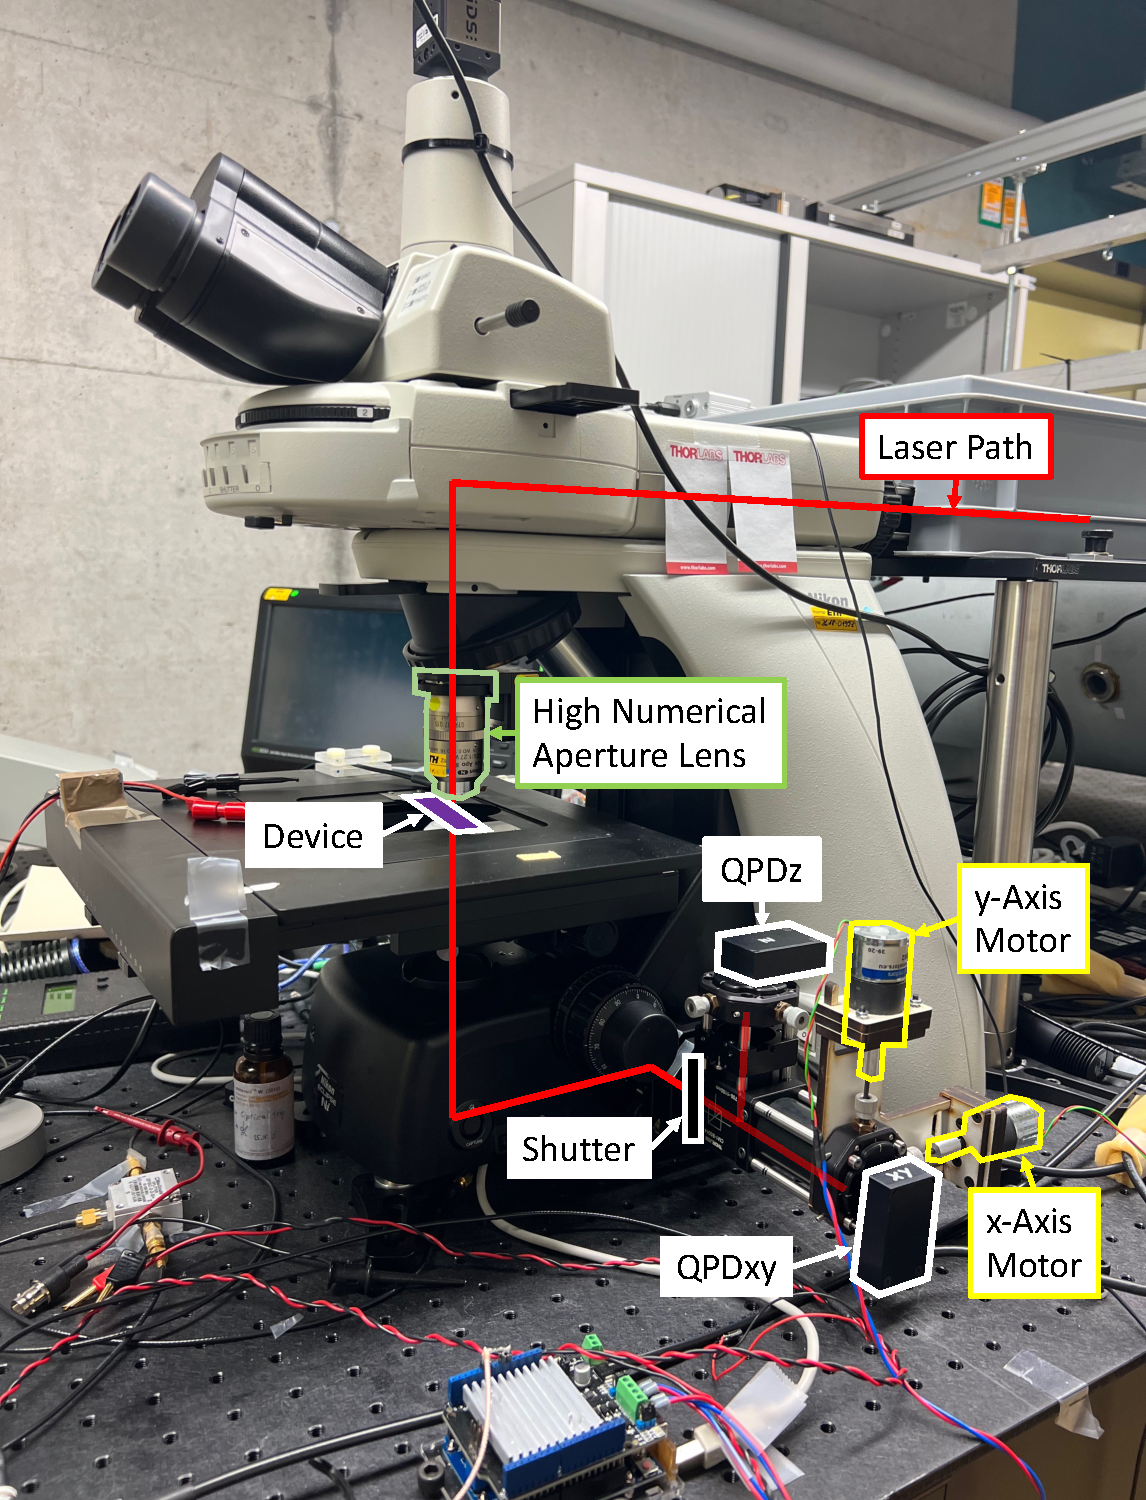
\includegraphics[width=0.8\textwidth]{SECTION/15_Figures/Supplemental_OT.pdf}
  \caption{Photograph of optical trapping setup with highlighted important 
  equipment.}
\end{figure*}

\newpage
\begin{figure*}[tbp]
  \centering
  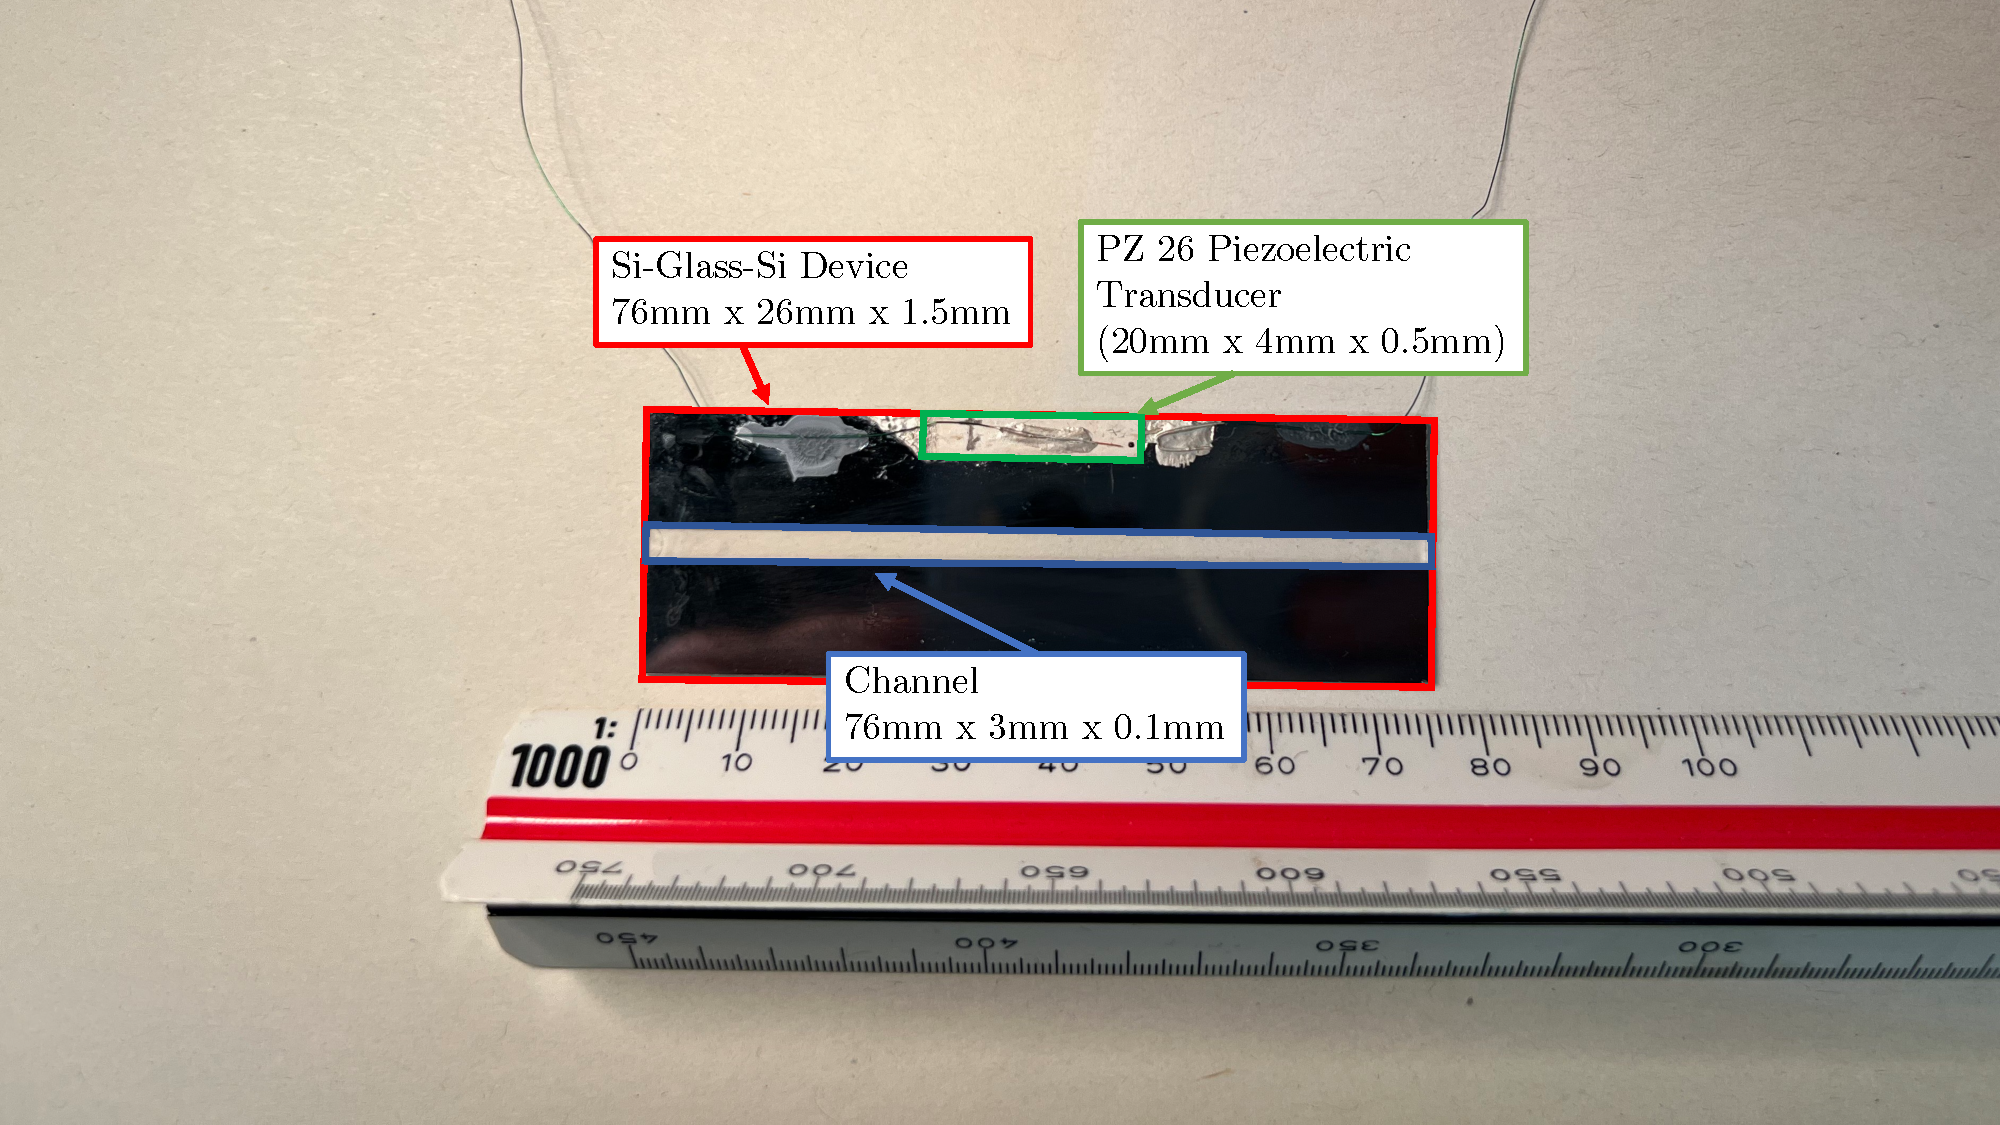
\includegraphics[width=\textwidth]{SECTION/15_Figures/Supplemental_Device.pdf}
  \caption{Photograph of acoustofluidic device.}
\end{figure*}

\newpage
\begin{figure*}[tbp]
  \centering
  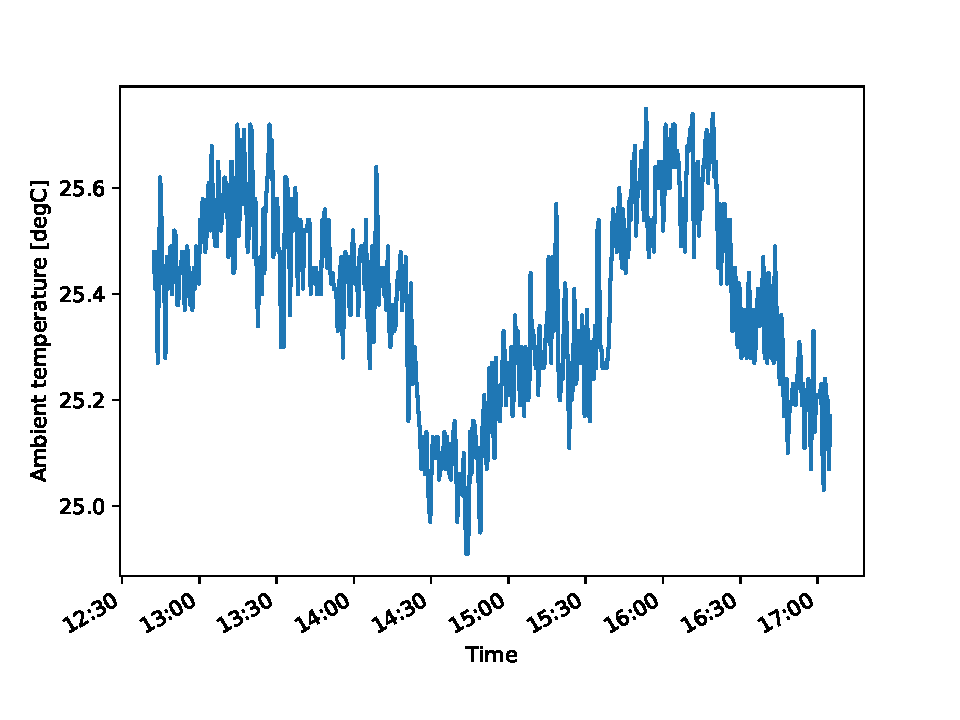
\includegraphics[width=\textwidth]{SECTION/15_Figures/temperature.pdf}
  \caption{Temperature at device for $k=1000$ BM series. The experiment of 80\% 
  occurred between 14:00 and 15:00.}
\end{figure*}

